\documentclass{csse4400}

% \teachermodetrue

\usepackage{float}

\usepackage{languages}

\title{Monitoring \& Events}
\author{Brae Webb}

\date{\week{6}}
\begin{document}

\maketitle

\begin{figure}[ht]
  \href{https://www.oreilly.com/library/view/designing-data-intensive-applications/9781491903063/ch11.html}{
    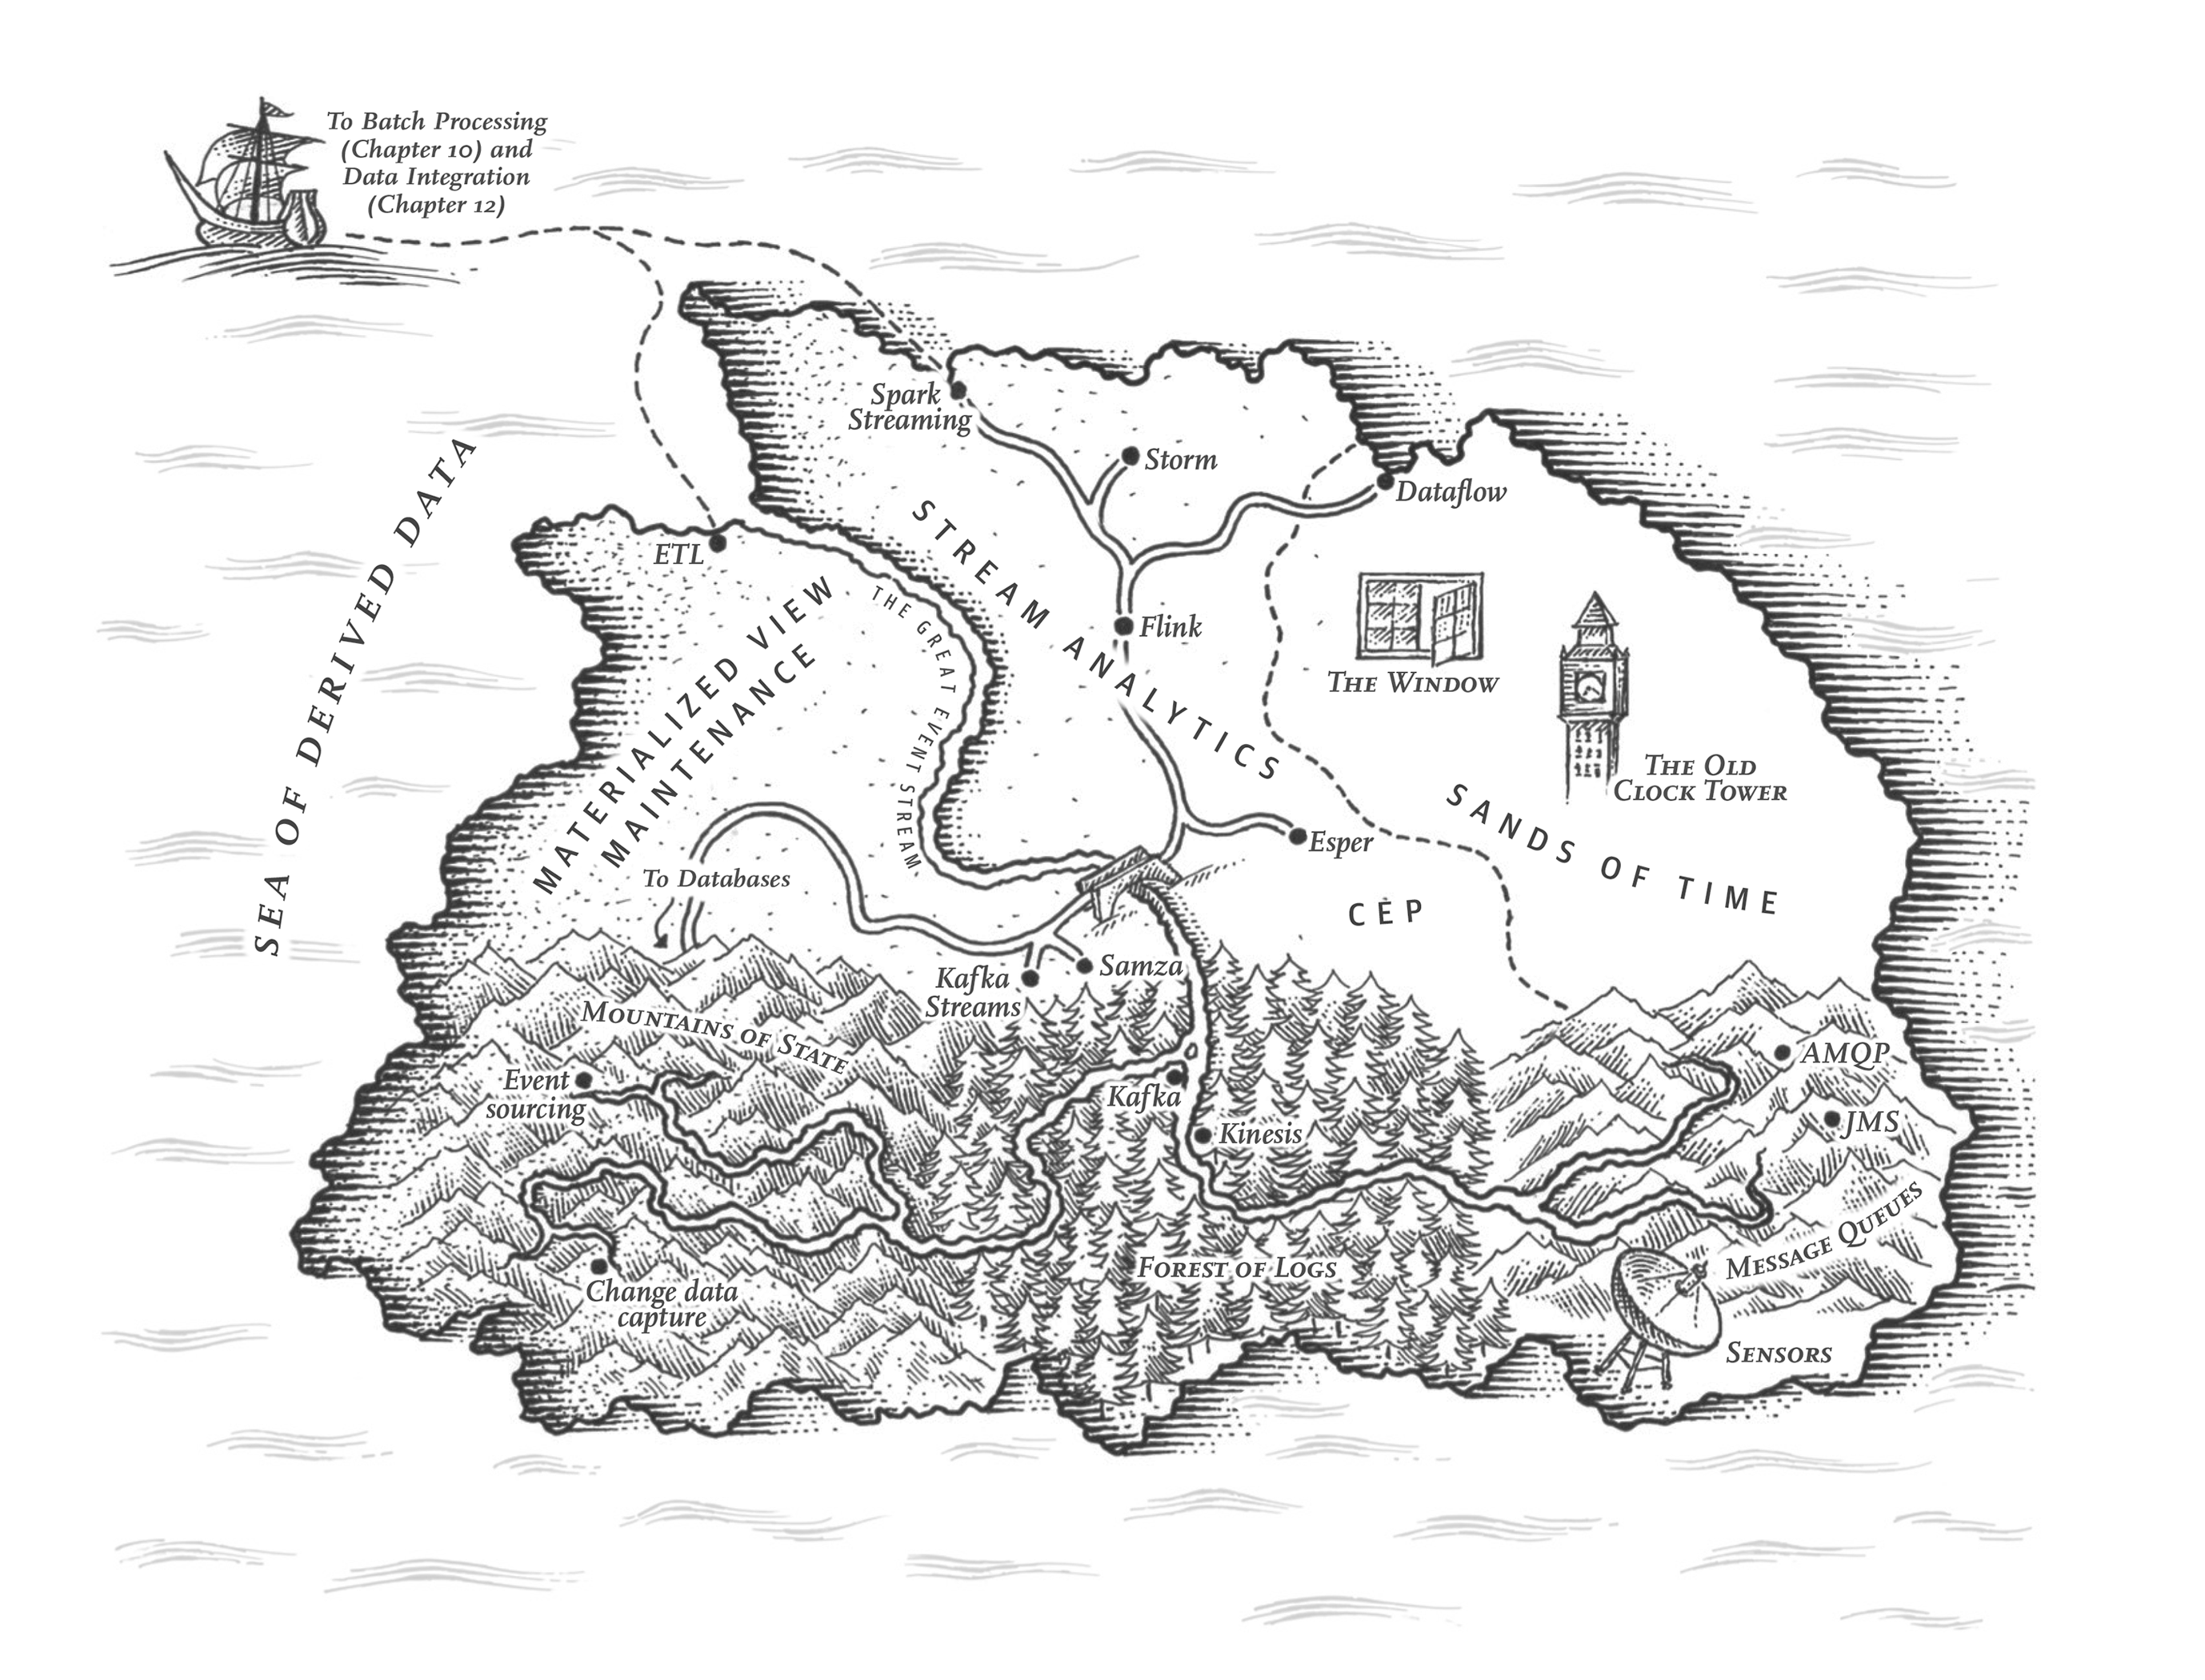
\includegraphics[width=\textwidth]{images/streams}
  }
\caption{A map of stream processing \cite{data-intensive}.}
\end{figure}

\section{This Week}
This week our goal is to:
\begin{itemize}
  \item investigate the various options to perform health-checks on services;
  \item explore the CloudWatch dashboard to monitor our services; and
  \item run an application that processes events asynchronously using SQS.
\end{itemize}


\section{Health-checks}

\teacher{
  Here we really just want to highlight that health-checks are the way in which container managers determine 
  whether or not to spin up or down an application.
  We should note that custom health-checks can be implemented to give application-specific ways of judging health.
}

Health-checks are a way to determine whether or not a service is healthy.
They are a core component to developing reliable and scalable systems.
Health-checks are utilized by systems that manage collections of service instances,
such as Kubernetes, Docker-compose, and of course, AWS Auto-scaling Groups.

In the context of AWS,
health-checks serve help load balancers route traffic only to healthy instances.
Additionally health-checks can instruct auto-scaling groups to spin down unhealthy instances and replace them with new healthy instances.

% There a few methods to determine whether a service is healthy or not.
% \subsection{Liveness checks}

% \subsection{Local health checks}

% \subsection{Dependency health checks}

% \subsection{Anomaly detection}

\section{CloudWatch}

\teacher{
  Here we want to introduce them to the interface of CloudWatch.
  If you have time to prep before perhaps run some service to show off logs.
  This is just a brief overview with some strong hinting that they might want to acquaint themselves with CloudWatch when doing the scalablity assignment and potentially the project.
}

CloudWatch is the AWS solution for monitoring services.
CloudWatch supports service metrics, logging, and alarms.
When working with AWS it is important to understand what CloudWatch can be used for.

\info{
  For the cloud assignment,
  we will be be testing that your submission is able to handle an appropriate load.
  We intend to be give notice of when this testing will occur.
  The use of CloudWatch to monitor your services and create alarms may give you the ability to manually recover from increased load and perform better in the assignment.
}

\subsection{Metrics}
Metrics are at the core of CloudWatch.
Metrics track important details about other AWS services often stored as time-series data.
For example, EC2 instances store metrics such as CPU and Memory usage.
While load balancers record metrics such as the amount of requests and amount of HTTP 200 responses.

Metrics help you to monitor and maintain services running on AWS.
When combined with Dashboards they are a powerful way to overview your systems.

\subsection{Alarms}
CloudWatch alarms can be configured to perform certain actions based on metrics.
For example, you may trigger an excessive amount of load balancer requests to increase the size of an auto-scaling group.
Or trigger an RDS instance with too little disk space to notify database admin.

\begin{code}[language=terraform]{}
resource "aws_cloudwatch_metric_alarm" "monitor_alb" {
  comparison_operator = "GreaterThanOrEqualToThreshold"
  metric_name         = "RejectedConnectionCount"
  namespace           = "AWS/ApplicationELB"
  period              = "120"
  statistic           = "Sum"
  threshold           = "10"

  dimensions = {
    LoadBalancer = aws_lb.balancer.name
  }

  alarm_description = "Increase auto-scaling capacity when 10 requests are rejected due to capacity limits"
  alarm_actions     = // increase auto-scaling group capacity.
}

resource "aws_cloudwatch_metric_alarm" "db_free_storage_space_warning" {
  comparison_operator = "LessThanThreshold"
  metric_name         = "FreeStorageSpace"
  namespace           = "AWS/RDS"
  period              = "120"
  statistic           = "Sum"
  threshold           = 10000000000 // 10 GB
  alarm_description   = "Free space dropped below 10 GB"
  alarm_actions       = // alert database adims
}
\end{code}

\teacher{
  Dear Evan Hughes,

  Commit messages such as `THings are happening' and `Oppsie Whoopie' may be the breaking point of my sanity.

  Much Love,
  
  Mr Webb
}

\noindent The entrypoint for understanding which metrics are available is:

\noindent \url{https://docs.aws.amazon.com/AmazonCloudWatch/latest/monitoring/aws-services-cloudwatch-metrics.html}

\subsection{Logging}
CloudWatch offers a logging end-point.
It can be utilized to log application data from EC2 instances.
For example, if you run an nginx server on an EC2 instance,
you can configure CloudWatch to process and store those logs.
This feature can be quite helpful and can be extended to the log files of applications you build.

In addition to being processing EC2 log files,
CloudWatch comes with built-in logging for some services.
For Lambda services it will log print statements or errors.
For application load balancer,
it will log detailed request information.
These logs are incredibly helpful for debugging.


\section{Event Processing}

As we saw in the Event-Driven Architecture notes \cite{events-notes},
event processing enable us to build highly scalable and extensible systems.
In this weeks practical we will get our hands dirty with event processing using AWS SQS.
SQS gives us a service which can act as an event broker.

\subsection{Technologies}

We should first discuss a few of our technology options for services which can be used in an Event-Driven Architecture.

% \info{
%   Below we only discuss external stream technologies but it is common to have streams within an application where concurrency is needed. 
%   Instead of dealing with concurrency using locking based methods like in CSSE2310, we can use streams to send data to the consumers that need to handle single writer usecases.
% }

\subsubsection{AWS SQS}

AWS provides the Simple Queue Service, SQS,
which offers a simple and fully managed message queue service.
There are two flavours of SQS to be aware of;
the standard message queue, and the FIFO message queue.
Standard message queues allow for greater scalability by providing higher through-put.
However, standard message queues in SQS are not exactly queues,
messages are not first in first out,
they are best-effort ordered.
The second flavour, FIFO message queues,
guarantees that messages are First in First Out.

\subsubsection{AWS SNS}

\subsubsection{AWS MQ / Apache ActiveMQ / RabbitMQ}

\aside{Not available in the lab environments}

\subsubsection{AWS MSK ( Managed Streaming for Apache Kafka )}

\aside{Not available in the lab environments}

\subsubsection{Redis}

\aside{Not available in the lab environments}

\section{Talking to the Simple Queue Service (SQS)}

\warning{
    For terminal examples in this section,
    lines that begin with a \$ indicate a line which you should type while the other lines are example output that you should expect.
    Not all of the output is captured in the examples to save on space.  
}

Today we will be creating and experimenting with the two queue flavours of AWS SQS.
A standard queue, named \texttt{csse6400\_prac} and a FIFO queue, named \texttt{csse6400\_prac.fifo}.
The Terraform code below can be used to create these two queues.

\info{
  If you have forgotten how to get started you will need to run the following commands in a local terminal.

  \bash{
    terraform init^^J
    ...^^J
    $ terraform plan^^J
    ...^^J
    $ terraform apply^^J
    ...
  }
}

\teacher{
  In the below terraform it is pretty simple and relies a lot on defaults.
  Though the FIFO name needs to have .fifo at the end, make sure to mention this.
}

\begin{code}[language=terraform, numbers=none]{}
terraform {
  required_providers {
    aws = {
      source = "hashicorp/aws"
      version = "~> 3.0"
    }
  }
}

provider "aws" {
  region = "us-east-1"
  shared_credentials_file = "./credentials"
}

resource "aws_sqs_queue" "our_first_mailbox" {
  name                        = "csse6400_prac"
}

resource "aws_sqs_queue" "our_first_fifo" {
  name                        = "csse6400_prac.fifo"
  fifo_queue                  = true
  content_based_deduplication = true
}

output "mailbox" {
  value = aws_sqs_queue.our_first_mailbox.arn
}

output "fifo" {
  value = aws_sqs_queue.our_first_fifo.arn
}
\end{code}

Now that we have provisioned the queues we can have a look at them in the AWS Console.
In the main AWS dashboard you can search for ``SQS'' to find these queues.
You should reach a page like this:

\begin{figure}[H]
  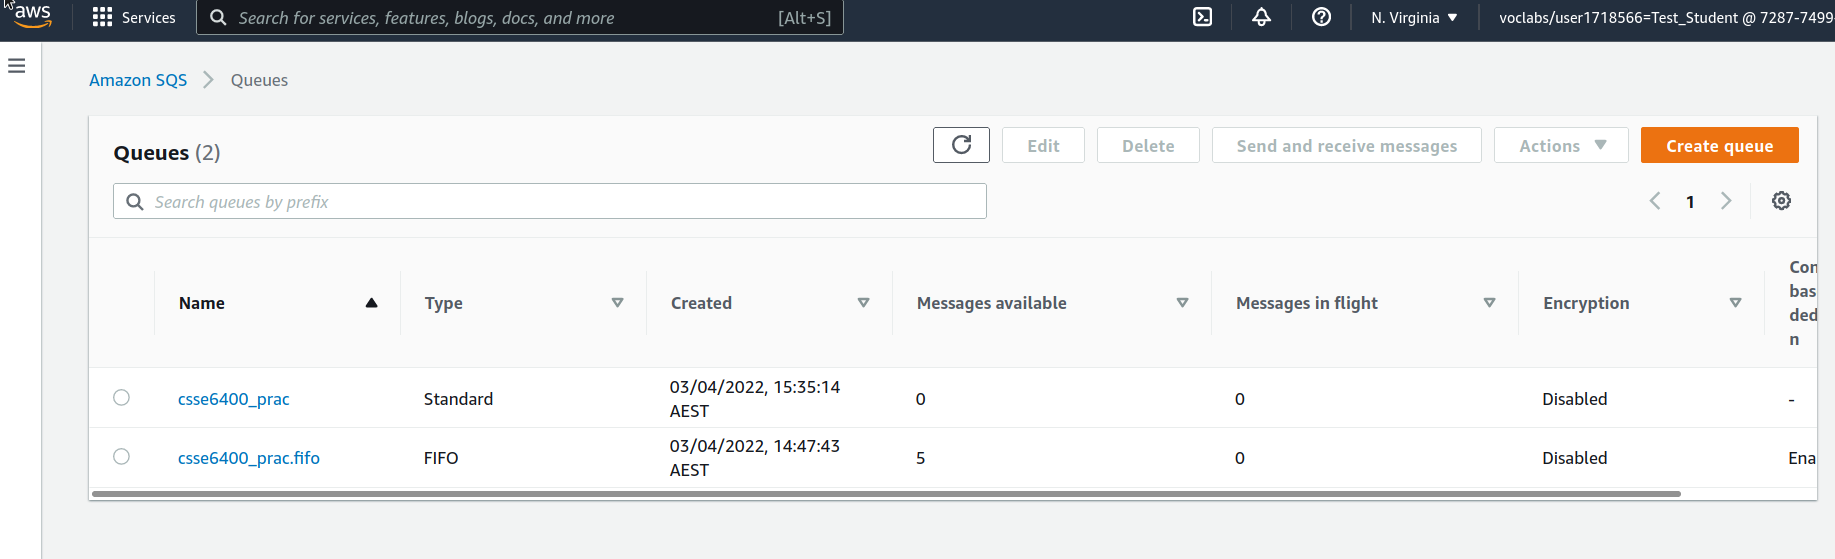
\includegraphics[width=\textwidth]{images/sqspanel}
\end{figure}

Like the EC2 and RDS dashboards,
we can browse the queue configurations and metrics.
  
\teacher{
  Show the students the Monitoring Panel and Access Policy panel in particular.

  \begin{itemize}
    \item Monitoring: Messages Sent/Received
    \item Monitoring: Empty Receives - This is the receiver getting nothing from polling. Costs \$ in the real world.
    \item Policy: Not covering today but SQS is a public service, it is protected via AWS credentials. In real use cases you need to configure a Access Policy.
  \end{itemize}
}

\subsection{Queue Command-line Interface}

We have provided a small docker container for you to use with your queues to see the differnce between the implementations.
First we must retrieve our AWS credentials and setup our environment.

With our learner lab grab the AWS credentials but instead of creating a credentials file we will be using environment variables.
Make a folder for the practi.

\begin{code}[language=shell, numbers=none]{}
$ mkdir queues && cd queues
\end{code}

Now we need to create an environment file for our docker container to read so that it can access AWS. Create a ``.env'' file in the current directory and edit the contents so that it looks similar to the below: The AWS keys will be from the credentials shown in your lab environment.

\begin{code}[numbers=none]{}
TERM=xterm-256color
AWS_ACCESS_KEY_ID=...
AWS_SECRET_ACCESS_KEY=...
AWS_SESSION_TOKEN=...
\end{code}

\begin{code}[numbers=none,keepspaces=true]{}
$ docker run --rm -it --env-file .env ghcr.io/csse6400/queue:main --name "test" --client-name "Client 1"


  __________
 |   \XX/   |
 | T. \/ .T |      University of Queensland
 | XX:  :XX |          Faculty of EAIT
 T L' /\ 'J T
  \  /XX\  /         CSSE6400 Queue Prac
@\_ '____' _/@       csse6400.uqcloud.net
\_X\_ __ _/X_/
 \=/\----/\=/



Unable to find a Queue by this name test
\end{code}

If your program shows the above then your ready to head to the next section :).
  

% \begin{code}[language=shell, numbers=none]{}
% docker run --rm -it --env-file .env ghcr.io/csse6400/queue:main --name "csse6400_prac" --client-name "hello" --sender
% \end{code}

% \begin{code}[language=shell, numbers=none]{}
%   docker run --rm -it --env-file .env ghcr.io/csse6400/queue:main --name "csse6400_prac" --client-name "hello" --sender
% \end{code}
  



\subsection{SQS Standard}

As we have stated above the ``Standard'' offering of SQS does not guarantee order or ``only once delivery''. 
Assuming our terraform was created sucessfully we are going to create one publisher and one subscriber.

\info{
  For the rest of this practical you will require multiple terminals. Make sure these are all in the same folder so we can reuse the .enf file. 
}

To create the subscriber run the following command:

\begin{code}[numbers=none,keepspaces=true]{}
  $ docker run --rm -it --env-file .env ghcr.io/csse6400/queue:main --name "csse6400_prac" --client-name "Client 1" --receive
\end{code}

\begin{figure}[H]
  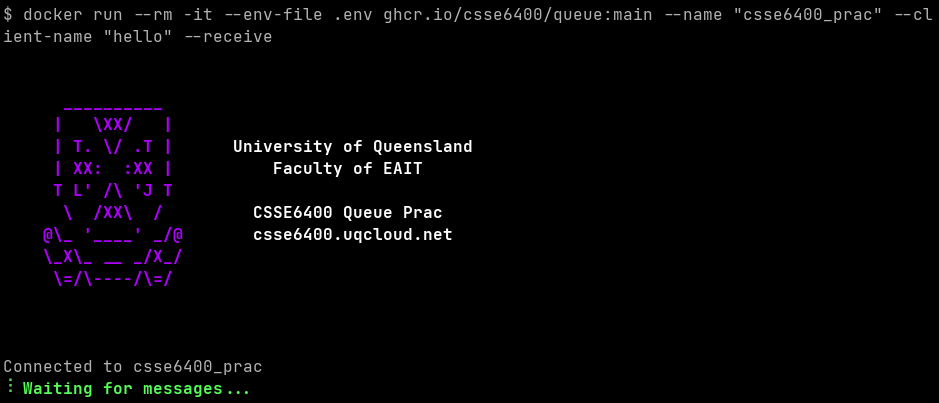
\includegraphics[width=\textwidth]{images/stacksub}
\end{figure}

Now lets start a publisher in another terminal but keep both terminals on your screen if you have space.

\begin{code}[numbers=none,keepspaces=true]{}
  $ docker run --rm -it --env-file .env ghcr.io/csse6400/queue:main --name "csse6400_prac" --client-name "Client 1"
\end{code}

\begin{figure}[H]
  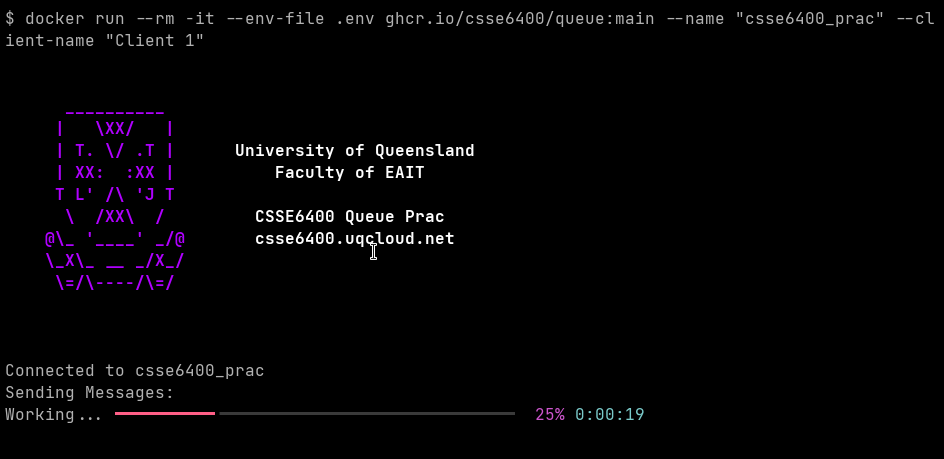
\includegraphics[width=\textwidth]{images/stackpub}
\end{figure}

When the publisher connects to the Queue it is going to put 100 messages of increasing increment into the queue. On the subscriber we will be able to see the messages being received, an example is provided below:

\begin{figure}[H]
  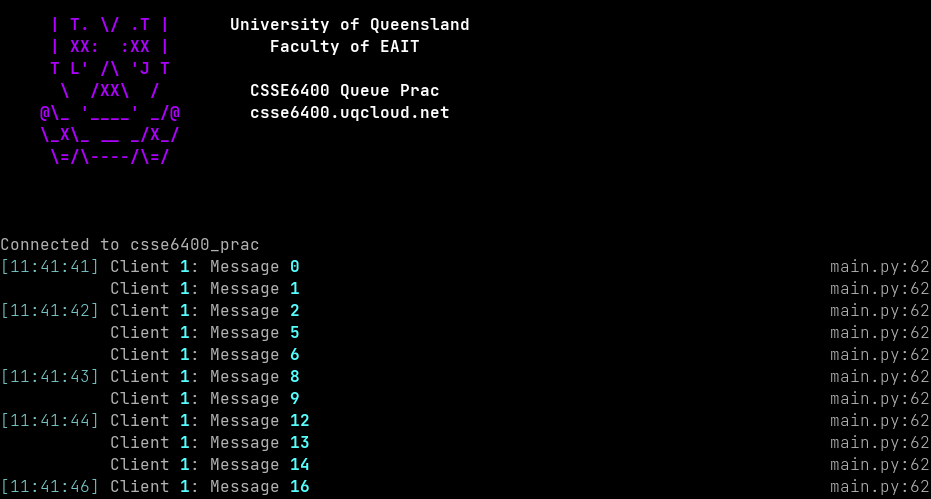
\includegraphics[width=\textwidth]{images/stacksubdata}
\end{figure}

hopefully like our example you can see that some of the messages arrive out of order. Next add more publishers and subscribers and experiment with the differnt configurations. 

\info{
  When making multiple publishes you may want to change the client-name cli parameter so you can keep track of when the messages arrived at the subscribers.
}


\subsection{SQS FIFO}
Now we will experiment with the FIFO based service offered by SQS. Like before we will start a subscriber but make sure the name of the queue matches the FIFO queue we created in terraform.

\begin{code}[numbers=none,keepspaces=true]{}
  $ docker run --rm -it --env-file .env ghcr.io/csse6400/queue:main --name "csse6400_prac.fifo" --client-name "Client 1" --receive
\end{code}

Now lets start a publisher in another terminal but keep both terminals on your screen if you have space.

\begin{code}[numbers=none,keepspaces=true]{}
  $ docker run --rm -it --env-file .env ghcr.io/csse6400/queue:main --name "csse6400_prac.fifo" --client-name "Client 1"
\end{code}

\begin{figure}[H]
  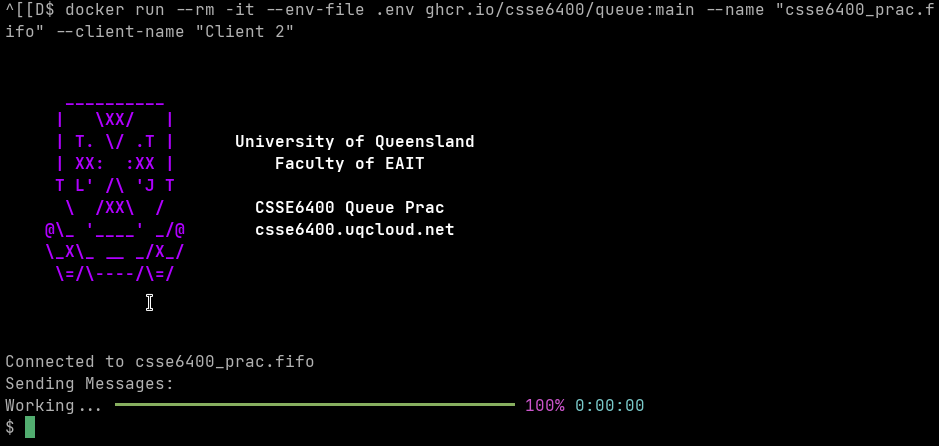
\includegraphics[width=\textwidth]{images/fifopub}
\end{figure}

On the subscriber we now see the messages arriving in order which is to be expected.

\begin{figure}[H]
  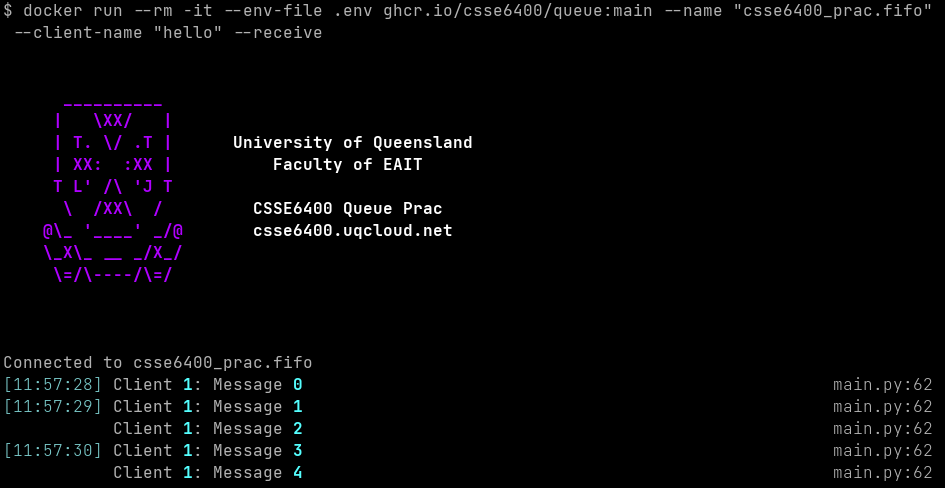
\includegraphics[width=\textwidth]{images/fifosub}
\end{figure}

If we re-run the publisher though we may not see any new messages make it to the consumer. This is because we have asked AWS to dedup messages where it can.

\teacher{
  Theres a cli param which prepends to the message to allow you to rerun if needed. It is --prepend "abcdef"
}

Again as before try experimenting with differnt publisher / subscriber configurations to see how they behave.

\info{
  When making multiple publishes you may want to change the client-name cli parameter so you can keep track of when the messages arrived at the subscribers.
}

\warning{
  \textbf{Please remember to terraform destroy to delete your resources}
}


\section{Optional Exercise: Worker Queues}

One good usecase of queues is for distributing work over many machines to scale to demand. In this exercise we encourage you to have a look at these widly used libraries to see how you could integrate them into a distributed system.

\begin{itemize}
  \item Python: \href{https://docs.celeryq.dev/en/stable/}{Celery}
  \item Java: \href{https://www.rabbitmq.com/tutorials/tutorial-one-java.html}{RabbitMQ}
\end{itemize}

The two above libraries are integrated into many of the popular application frameworks aswell.

\bibliographystyle{ieeetr}
\bibliography{books,ours}

\end{document}